\documentclass{beamer}
\usepackage[utf8]{inputenc}
\usepackage{musicography}
\usepackage{graphicx}

% images
\usepackage[export]{adjustbox}
\usepackage{caption}

%% doc deets
\title{The Order of Mathematistry}
\subtitle{Queering metascience with mathematics}
\titlegraphic{
%\vspace{-5cm}
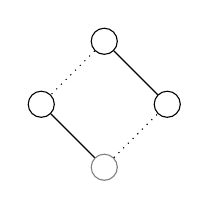
\begin{tikzpicture}[scale=0.8]

% nodes
\node [ style = hassenode] (f) {};
\node[style = hassenode] (g) at (-1, -1) {};
\node [style = hassenode] (h) at (1, -1) {};
\node [style = hassenode, gray] (i) at (0, -2) {};

%  edges
\draw [dotted] (f) to (g);
\draw (g)  to (i);
\draw [dotted] (i) to (h);
\draw (h) to (f);
%\vspace{5cm}
\end{tikzpicture}
}
\author{Charles T. Gray^{$\musEighth$}\\ Hannah Fraser, Hien Nguyen, \\Elise Gould, and Danielle Navarro}
\institute{$\musEighth$\ Reproducibility team, The repliCATS Project \\Interdisciplinary Metaresearch Group, University of Melbourne}

\date{February 2020}


% general packages
\usepackage{amssymb, amsthm, amsmath}

% biblio
\usepackage[url=false]{biblatex}
\addbibresource{references.bib}
%\renewcommand*{\bibfont}{\scriptsize}
\renewcommand*{\bibfont}{\tiny}

% itemised list
\usepackage{enumitem}

% tikz
\usepackage{tikz}
\usetikzlibrary[shapes,arrows]
\tikzset{hassenode/.style={circle,draw}}
\usepackage{adjustbox} % resize by height

% code macros
\newcommand{\code}[1]{\texttt{#1}}
\newcommand{\package}[1]{\texttt{#1::}}

% fix hyphenation issues
\usepackage{csquotes}
\usepackage[british]{babel} % hopefully this fixes some of the hyphenation issues
\hyphenation{re-pro-du-ci-bility}
\hyphenation{pre-reg-istration}


% beamer specs
\beamertemplatenavigationsymbolsempty{}
\setbeamertemplate{footline}[frame number]

\usefonttheme{serif}
\setbeamercolor*{structure}{fg= darkgray}

%\setbeamercolor*{palette tertiary}{fg=black,bg=black!10}
%\setbeamercolor*{palette quaternary}{fg=black,bg=black!10}

%\setbeamercolor*{lower separation line head}{bg=orange}
\AtBeginSection[]{\frame{\frametitle{Outline}%
\tableofcontents[currentsection,hideothersubsections]}}%

\usebackgroundtemplate{
\includegraphics[width=\paperwidth,height=\paperheight]{parchment.jpg}}

% theorem environment
\usepackage{thmtools}

\declaretheoremstyle{qthmstyle}
\declaretheorem[style=qthmstyle,name=Proposition]{proposition}
\declaretheorem[style=qthmstyle,name=Definition]{defn}
%\declaretheorem[style=qthmstyle,name=Theorem]{theorem}
%\declaretheorem[style=qthmstyle,name=Lemma]{lemma}
%\declaretheorem[style=qthmstyle,name=Corollary]{corollary}




%%
\begin{document}



% title frame
\begin{frame}

\maketitle

\end{frame}

\section{A value judgement is, after all, an order}


\begin{frame}{Queering literature}

\begin{centering}
\begin{columns}

\begin{column}{0.5\textwidth}


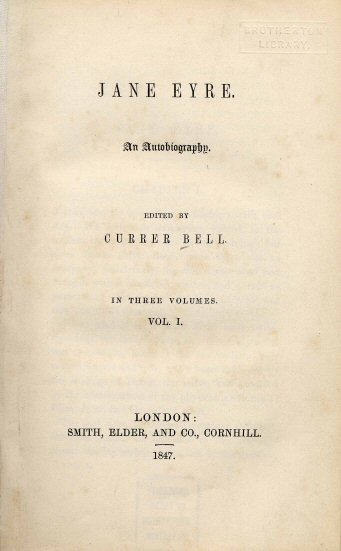
\includegraphics[scale=1.2]{Jane_Eyre_title_page.jpg}
\medskip

\small{
\emph{Jane Eyre}, 1847

\medskip

Charlotte Bront\"e~\cite{bronte2000jane}
}

\end{column}

\begin{column}{0.5\textwidth}


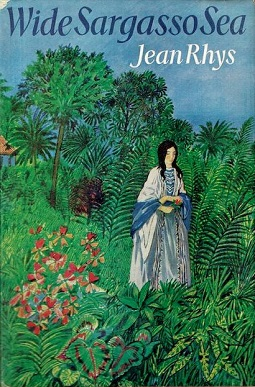
\includegraphics[scale=0.55]{JeanRhys_WideSargassoSea.jpg}
\medskip

\small{
\emph{Wide Sargasso Sea}, 1966

\medskip

Jean Rhys~\cite{rhys1992wide}
}


\end{column}

\end{columns}

\begin{flushright}
\tiny{Image sources: Wikipedia.}
\end{flushright}


% \begin{flushright}
% 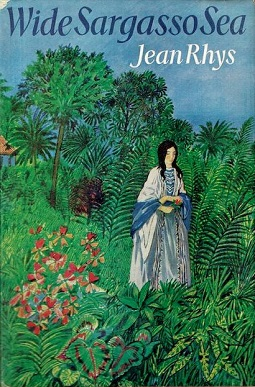
\includegraphics[scale=0.6]{JeanRhys_WideSargassoSea.jpg}

% \tiny{Image source: Wikipedia}
% \end{flushright}

% \emph{Wide Sargasso Sea}, Jean Rhys, 1966

% \bigskip
\end{centering}

\end{frame}

\begin{frame}{Queering metascience}

    \begin{quote}
        So let’s build an open and reproducible science as a queer reimagining of science and not a small perturbation of the world that is. Such a system will never be perfect.
    \end{quote}

\begin{flushright}
-- Dan Simpson~\cite{simpson_what_2019}
\end{flushright}

\end{frame}

\begin{frame}{Preregistration is redundant, at best}

The Centre for Open Science defines \textbf{preregistration} as specifying the research plan in advance~\cite{centre_for_open_science_preregistration_2020}.

\vspace{1cm}

2019: Preregistration is Hard, and Worthwhile, Nosek \emph{et al.}~\cite{nosek_preregistration_2019}

\vspace{1cm}

2019: Is Preregistration Worthwhile? Szollosi \emph{et al.}~\cite{szollosi_preregistration_2019}

\bigskip

\begin{quote}
The diagonisticity of statistical tests depend entirely on how well statistical models map onto underlying theories, and so improving statistical techniques does little improve theories \underline{when the mapping is weak}~\cite{szollosi_preregistration_2019}.
\end{quote}


\end{frame}

\begin{frame}{Mathematistry}
Navarro, a mathematical scientist specialising in psychology, redefines Box's term \textbf{mathematistry}~\cite{box_science_1976} to

\bigskip

\begin{quote}
`describe using formal tools to define a statistical problem that differs from the
scientific one, solving the redefined problem, and declaring the scientific concern addressed'~\cite{navarro_between_2018}.
\end{quote}

\bigskip

We will think of \textbf{mathematistry} as the measure of strength of mapping to describe \underline{when the mapping is weak}~\cite{szollosi_preregistration_2019}.


\end{frame}

%%% Order
\begin{frame}{A value judgement is, after all, an order}
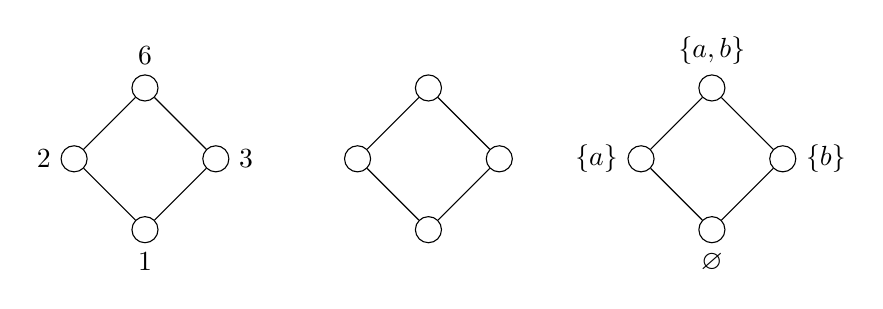
\begin{tikzpicture}[scale = 0.9]

\begin{scope}[xshift=0cm]

  % nodes

  \node [ style = hassenode, label=above:6] (f) {};
  \node[style = hassenode, label=left:2] (g) at (-1, -1) {};
  \node [style = hassenode, label=right:3] (h) at (1, -1) {};
  \node [style = hassenode, label=below:1] (i) at (0, -2) {};

  %  edges
  \draw [] (f) to (g);
  \draw (g)  to (i);
  \draw [] (i) to (h);
  \draw (h) to (f);

  \end{scope}

\begin{scope}[xshift=4cm]

% nodes
\node [ style = hassenode] (f) {};
\node[style = hassenode] (g) at (-1, -1) {};
\node [style = hassenode] (h) at (1, -1) {};
\node [style = hassenode] (i) at (0, -2) {};

%  edges
\draw [] (f) to (g);
\draw (g)  to (i);
\draw [] (i) to (h);
\draw (h) to (f);

\end{scope}

\begin{scope}[xshift=8cm]

% nodes

  \node [ style = hassenode, label=above:{\(\{a,b\}\)}] (f) {};
  \node[style = hassenode, label=left:{\(\{a\}\)}] (g) at (-1, -1) {};
  \node [style = hassenode, label=right:{\(\{b\}\)}] (h) at (1, -1) {};
  \node [style = hassenode, label=below:{\(\varnothing\)}] (i) at (0, -2) {};

%  edges
\draw [] (f) to (g);
\draw (g)  to (i);
\draw [] (i) to (h);
\draw (h) to (f);

\end{scope}

\end{tikzpicture}
\end{frame}



%%%  Heuristics

\section{Heuristics of mathematistry}


\begin{frame}{Heuristics of mathematistry}
\begin{center}
\begin{tikzpicture}[scale = 0.9]
\begin{scope}

%  nodes
\node [style = hassenode] (a) at (0,0) {};
\node [style = hassenode] (b) at (0,-2) {};

% edges
\draw (a) to (b);
\end{scope}

%\end{tikzpicture}

%\begin{tikzpicture}

\begin{scope}[xshift=4cm]

% nodes
\node [style = hassenode, gray] (c) at (0,0) {};
\node [style = hassenode] (d) at (0,-1) {};
\node [style = hassenode, gray] (e) at (0, -2) {};

% edges
\draw [dotted] (c) to (d);
\draw [dotted] (d) to (e);
\end{scope}

\begin{scope}[xshift=8cm]

% nodes
\node [ style = hassenode] (f) {};
\node[style = hassenode] (g) at (-1, -1) {};
\node [style = hassenode] (h) at (1, -1) {};
\node [style = hassenode, gray] (i) at (0, -2) {};

%  edges
\draw [dotted] (f) to (g);
\draw (g)  to (i);
\draw [dotted] (i) to (h);
\draw (h) to (f);

\end{scope}

\end{tikzpicture}
\end{center}


\end{frame}

\begin{frame}{Heuristics of mathematistry}


% \onslide<2>

A heuristic can be thought of in terms of a mapping from \(C \times M\) to some space of measuring how well a pairing `furthers the process of scientific discovery' (Devezer \emph{et al., 2019})~\cite{devezerScientificDiscoveryModelcentric2019}.

\vspace{2cm}

\(\texttt{fpd}\) := furthers the process of scientific discovery


\end{frame}

\begin{frame}{Heuristics of mathematistry}
  \begin{center}
  \begin{tikzpicture}[scale = 0.9]
  \begin{scope}

  %  nodes
  \node [style = hassenode] (a) at (0,0) {};
  \node [style = hassenode] (b) at (0,-2) {};

  % edges
  \draw (a) to (b);
  \end{scope}

  %\end{tikzpicture}

  %\begin{tikzpicture}

  \begin{scope}[xshift=4cm]

  % nodes
  \node [style = hassenode, gray] (c) at (0,0) {};
  \node [style = hassenode] (d) at (0,-1) {};
  \node [style = hassenode, gray] (e) at (0, -2) {};

  % edges
  \draw [dotted] (c) to (d);
  \draw [dotted] (d) to (e);
  \end{scope}

  \begin{scope}[xshift=8cm]

  % nodes
  \node [ style = hassenode] (f) {};
  \node[style = hassenode] (g) at (-1, -1) {};
  \node [style = hassenode] (h) at (1, -1) {};
  \node [style = hassenode, gray] (i) at (0, -2) {};

  %  edges
  \draw [dotted] (f) to (g);
  \draw (g)  to (i);
  \draw [dotted] (i) to (h);
  \draw (h) to (f);

  \end{scope}

  \end{tikzpicture}
  \end{center}

  \small{
  \[
  h: C \times M \to \begin{cases}
                  \{0, 1\} & \text{if \(\texttt{fpd}\) or not;}\\
                  [0, 1] & \text{if \(\texttt{fpd}\) on a spectrum;}\\
                  H & \text{if \(\texttt{fpd}\) otherwise}.
              \end{cases}
  \]
  }

\end{frame}


\begin{frame}{Heuristics of mathematistry}

Let \(C\) denote the set of all possible \textbf{scientific claims} for which we might provide evidence of, with a scientific method or procedure.

\bigskip

Let \(M\) denote the set of all possible \textbf{scientific methods} that can be used to provide evidence of scientific claims.

\bigskip

The product \(C \times M\) denotes the collection of possible \textbf{pairings of claim and methodology}.

\end{frame}

\begin{frame}{Heuristic of mathematistry}

\begin{definition} A \textbf{heuristic \(h\) of mathematistry} measures the efficacy of a pairing \((c,m)\) of scientific claim \(c \in C\), and method  \(m \in M\) of providing evidence of that claim, measuring how effective method \(m\) is at scientifically informing claim \(c\).

\vspace{1cm}

We denote $\mathbb H$ to be the set of all possible heuristics of mathematistry. For a heuristic $h$ in $\mathbb H$, we define the value $h(c,m)$ as the \textbf{measure of mathematistry} of pairing $(c,m)$ under heuristic $h$.
\end{definition}

\end{frame}

\begin{frame}{A value judgement on \emph{good enough}~\cite{wilson_good_2017} science}

\begin{center}
\begin{tikzpicture}[scale = 0.7]
\begin{scope}

%  nodes
\node [style = hassenode, label=above right:{$\top$}] (a) at (0,0) {};
\node [style = hassenode, label=below right:{$\bot$}] (b) at (0,-2) {};

% edges
\draw (a) to (b);
\end{scope}

%\end{tikzpicture}

%\begin{tikzpicture}

\begin{scope}[xshift=4cm]

% nodes
\node [style = hassenode, gray, label=above right:{\textcolor{gray}{$\top$}}] (c) at (0,0) {};
\node [style = hassenode] (d) at (0,-1) {};
\node [style = hassenode, gray,label=below right:{\textcolor{gray}{$\bot$}}] (e) at (0, -2) {};

% edges
\draw [dotted] (c) to (d);
\draw [dotted] (d) to (e);
\end{scope}

\begin{scope}[xshift=8cm]

% nodes
\node [ style = hassenode, label=above right:{$\top$}] (f) {};
\node[style = hassenode] (g) at (-1, -1) {};
\node [style = hassenode] (h) at (1, -1) {};
\node [style = hassenode, gray, label=below right:{\textcolor{gray}{$\bot$}}] (i) at (0, -2) {};

%  edges
\draw [dotted] (f) to (g);
\draw (g)  to (i);
\draw [dotted] (i) to (h);
\draw (h) to (f);

\end{scope}

\end{tikzpicture}
\end{center}

\bigskip

For a heuristic $h$ to be a member of $\mathbb H$, there must exist a scientific method $m$, and two distinct scientific claims we might reasonably pair $m$ with, $c_1$ and $c_2$, such that
$$
h(c_1,m) <  h(c_2,m)
$$
or, conversely, there must exist distinct methods, $m_1$ and $m_2$, such that, for a claim $c$, we have
$$
h(c, m_1) < h(c, m_2).
$$



\end{frame}



%%% Order operation

\begin{frame}{A relational operator of mathematistry}

\begin{definition}\label{def:om}
Let $(c_1, m_1) \to_h (c_2, m_2)$ if and only if $h(c_1, m_1) \leqslant h(c_2, m_2)$ under heuristic $h$ of mathematistry.
\end{definition}



\end{frame}


\section{The order of mathematistry}

%%% Order definition

\begin{frame}{Order}

To be considered an order, $\to_h$ must satisfy three properties~\cite{davey_introduction_2002-1}.

\vspace{1.5cm}

\begin{defn}\label{def:order}
A binary relation $\leqslant$ on set $P$ is an \textbf{order} if, for all $x, y, z \in P$, we have
\begin{enumerate}[label=(\roman*)]
    \item $x \leqslant x$,
    \item $x \leqslant y$ and $y \leqslant x$ implies $x = y$,
    \item $x \leqslant y$ and $y \leqslant z$ imply $x \leqslant z$.
\end{enumerate}

\end{defn}

\end{frame}


%%% Order definition

\begin{frame}{Order}

\begin{description}%[label=(\roman*)]
    \item[(i) reflexivity] $x \leqslant x$,
    \item[(ii) antisymmetry] $x \leqslant y$ and $y \leqslant x$ implies $x = y$,
    \item[(iii) transitivity] $x \leqslant y$ and $y \leqslant z$ imply $x \leqslant z$.
\end{description}

\vspace{1.5cm}

When a binary relation satisfies (i) reflexivity and (iii) transitivity, but not (ii) antisymmetry, we say it is a \textbf{quasi-order}.


 \end{frame}

\begin{frame}{A quasi-order of mathematistry}

 \begin{definition}
 When a binary relation satisfies (i) reflexivity and (iii) transitivity, but not (ii) antisymmetry, we say it is a \textbf{quasi-order}.
 \end{definition}

\vspace{1cm}

 Let $\mathcal X \subseteq C \times M$ denote the subset $\mathcal X$ of reasonable pairings $C \times M$ of claims and methods.

 \bigskip

    \begin{lemma}\label{lem:quasi}
The relation $\to_h$ is a quasi-order on $\mathcal X$.
\end{lemma}
\end{frame}

\begin{frame}{Partitions of mathematistry}

Define the equivalence class of mathematistry generated by a reasonable pairing, $(c,m) \in \mathcal X$,
$$
[[c,m]]_h := \{(x,y) \in \mathcal X \ | \ h(x,y) = h(c,m)\}.
$$

\bigskip

We then have reasonable pairings, $\mathcal X$, partitioned by mathematistry,
$$\mathfrak X_h := \mathcal X/_{\to_h}.$$


\end{frame}

\begin{frame}{The Order of Mathematistry}

The relation $\to_h$ is a quasi-order on $\mathcal X$, only satisfying reflexivity and transitivity, but not antisymmetry.

\bigskip

It can be shown that $\to_h$ on $\mathfrak X_h$ satisfies reflexivity, antisymmetry, and transitivity.

\end{frame}



\begin{frame}

\begin{theorem}
The relation $\to_h$ is an order on $\mathfrak X_h$.
\end{theorem}

\bigskip

\begin{definition}\label{def: mathy}
We refer to

\medskip

$$
\langle \mathfrak X; \to \rangle_h := \langle \mathcal X/\to_h ; \to_h \rangle
$$

\medskip

as the \textbf{order of mathematistry} under heurisic $h \in \mathbb H$.
\end{definition}



\end{frame}


%%% Section cardinality
\section{A question of cardinality}

\begin{frame}{A question of cardinality}

\begin{adjustbox}{max totalsize={.9\textwidth}{.9\textheight},center}
\begin{tikzpicture}
%%%  nodes

% hasse nodes
\node [circle, draw, gray, label=above right:{$[[\top]]_h$}] (a) at (0,0) {};
\node [circle, draw, gray, label=below right:{$[[\bot]]_h$}] (b) at (0,-8) {};
\node [circle, draw, gray, label=below right:{$[[\varnothing]]_h$}] (c) at (0, -10) {};

% heuristic nodes
\node  (h1) at (-4,-4) {};
\node [label=right:\textcolor{gray}{$\Tilde h$}] (h2) at (4, -4) {};
\node [circle, draw, gray] (w) at (-1,-3.1) {};

% representative nodes

% set label nodes
\node at (2.5, -7) {\textcolor{gray}{\footnotesize{$\langle C \times M ; \to \rangle_h$}}};
\node at (1.8, -6) {\textcolor{gray}{\footnotesize{$\langle \mathfrak X; \to \rangle_h$}}};
\node at (0, -2) {\footnotesize{$\langle \mathfrak P; \to \rangle_h$}};
\node at (-.8, -4) {\footnotesize{$\langle \mathfrak W; \to \rangle_h$}};

%%% edges

% underlying lattice
\draw (c) [gray] to (b);

% C x M
\draw (a) [out=-15, in=15, dotted, gray] to (b);
\draw (a) [out=-165, in=165, dotted, gray] to (b);

% X
\draw (a) [out=-45, in=45, densely dotted, gray] to (b);
\draw (a) [out=-135, in=135, densely dotted, gray] to (b);

% P
\draw (a) [
%out=-70, in=70, 
loosely dashed] to (b);
\draw (a) [out=-110, in=110, loosely dashed] to (b);

% W
\draw (w) [out=-45, in=45, densely dashdotted] to (b);
\draw (w) [out=-125, in=125, densely dashdotted] to (b);

% heuristic connect
\draw (h1) [out = 30, in = 150, loosely dotted] to (h2);
\end{tikzpicture}
\end{adjustbox}
\end{frame}

\section{A question of density}

\begin{frame}{\large{Are there distinct differences between classes of mathematistry?}}
 
\begin{adjustbox}{max totalsize={.9\textwidth}{.8\textheight},center}
\begin{tikzpicture}
%%%  nodes

% hasse nodes
\node [circle, draw, gray, label=above right:{$[[\top]]_h$}] (a) at (0,0) {};
\node [circle, draw, gray, label=below right:{$[[\bot]]_h$}] (b) at (0,-8) {};
\node [circle, draw, gray, label=below right:{$[[\varnothing]]_h$}] (c) at (0, -10) {};

% heuristic nodes
\node  (h1) at (-4,-4) {};
\node [label=right:\textcolor{gray}{$\Tilde h$}] (h2) at (4, -4) {};
\node [circle, draw, gray] (w) at (-1,-3.1) {};

% representative nodes

% set label nodes
\node at (2.5, -7) {\textcolor{gray}{\footnotesize{$\langle C \times M ; \to \rangle_h$}}};
\node at (1.8, -6) {\textcolor{gray}{\footnotesize{$\langle \mathfrak X; \to \rangle_h$}}};
\node at (0, -2) {\footnotesize{$\langle \mathfrak P; \to \rangle_h$}};
\node at (-.8, -4) {\footnotesize{$\langle \mathfrak W; \to \rangle_h$}};

%%% edges

% underlying lattice
\draw (c) [gray] to (b);

% C x M
\draw (a) [out=-15, in=15, dotted, gray] to (b);
\draw (a) [out=-165, in=165, dotted, gray] to (b);

% X
\draw (a) [out=-45, in=45, densely dotted, gray] to (b);
\draw (a) [out=-135, in=135, densely dotted, gray] to (b);

% P
\draw (a) [
%out=-70, in=70, 
loosely dashed] to (b);
\draw (a) [out=-110, in=110, loosely dashed] to (b);

% W
\draw (w) [out=-45, in=45, densely dashdotted] to (b);
\draw (w) [out=-125, in=125, densely dashdotted] to (b);

% heuristic connect
\draw (h1) [out = 30, in = 150, loosely dotted] to (h2);
\end{tikzpicture}
\end{adjustbox}
\end{frame}

\begin{frame}{A question of density}

\centering
 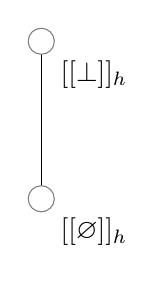
\begin{tikzpicture}

 %%%  nodes

 % hasse nodes
 %\node [circle, draw, gray, label=above right:{$[[\top]]_h$}] (a) at (0,0) {};
 \node [circle, draw, gray, label=below right:{$[[\bot]]_h$}] (b) at (0,0) {};
 \node [circle, draw, gray, label=below right:{$[[\varnothing]]_h$}] (c) at (0,-2) {};

 \draw (b) to (c);

 \end{tikzpicture}

\end{frame}

\section{The utility of heuristics}

\begin{frame}{The limitations of heuristics}
\begin{adjustbox}{max totalsize={.9\textwidth}{.8\textheight},center}
\begin{tikzpicture}
%%%  nodes

% hasse nodes
\node [circle, draw, gray, label=above right:{$[[\top]]_h$}] (a) at (0,0) {};
\node [circle, fill=gray, draw, gray, label=below right:{$[[\bot]]_h$}] (b) at (0,-8) {};
\node [circle, fill=gray, draw, gray, label=below right:{$[[\varnothing]]_h$}] (c) at (0, -10) {};

% heuristic nodes
\node  (h1) at (-4,-4) {};
\node [label=right:\textcolor{gray}{$\Tilde h$}] (h2) at (4, -4) {};
\node [circle, draw, gray] (w) at (-1,-3.1) {};

% representative nodes

% set label nodes
\node at (2.5, -7) {\textcolor{gray}{\footnotesize{$\langle C \times M ; \to \rangle_h$}}};
\node at (1.8, -6) {\textcolor{gray}{\footnotesize{$\langle \mathfrak X; \to \rangle_h$}}};
\node at (0, -2) {\footnotesize{$\langle \mathfrak P; \to \rangle_h$}};
\node at (-.8, -4) {\footnotesize{$\langle \mathfrak W; \to \rangle_h$}};

%%% edges

% underlying lattice
\draw (c) [gray] to (b);

% C x M
\draw (a) [out=-15, in=15, dotted, gray] to (b);
\draw (a) [out=-165, in=165, dotted, gray] to (b);

% X
\draw (a) [out=-45, in=45, densely dotted, gray] to (b);
\draw (a) [out=-135, in=135, densely dotted, gray] to (b);

% P
\draw (a) [
%out=-70, in=70, 
loosely dashed] to (b);
\draw (a) [out=-110, in=110, loosely dashed] to (b);

% W
\draw (w) [out=-45, in=45, densely dashdotted] to (b);
\draw (w) [out=-125, in=125, densely dashdotted] to (b);

% heuristic connect
\draw (h1) [out = 30, in = 150, loosely dotted] to (h2);
\end{tikzpicture}
\end{adjustbox}    
    
    
\end{frame}

\begin{frame}{The order of mathematistry on statistics}

\centering

 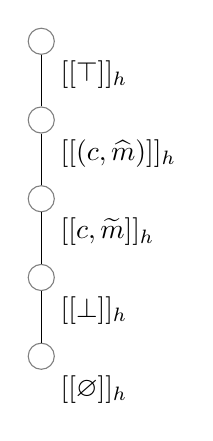
\begin{tikzpicture}

 %%%  nodes

 % hasse nodes
 \node [circle, draw, gray, label=below right:{$[[\top]]_h$}] (a) {};
 \node [circle, draw, gray, below of=a, label=below right:{$[[(c,\widehat m)]]_h$}] (b) {};
 \node [circle, draw, gray, below of=b, label=below right:{$[[c, \widetilde m]]_h$}] (c) {};
 \node [circle, draw, gray, below of=c, label=below right:{$[[\bot]]_h$}] (d) {};
 \node [circle, draw, gray, below of=d, label=below right:{$[[\varnothing]]_h$}] (e) {};

 \draw (a) to (b);
 \draw (b) to (c);
 \draw (c) to (d);
 \draw (d) to (e);

 \end{tikzpicture}

\end{frame}

\begin{frame}{\large{The order of mathematistry on QRPs in ecological models}}

\begin{adjustbox}{max totalsize={.9\textwidth}{.9\textheight},center}
\begin{tikzpicture}%[node distance = 3cm]
  [node distance=3cm,scale=0.65, every node/.style={transform shape}]

%%%  nodes

% hasse nodes

% top
\node [circle, draw, gray, label=below right:{$[[\top]]_h$}] (a) {};

% next from top
\node [circle, draw, gray, below of=a, label=above right:{$[[(c,m)]]_h$}] (b) {};

% one case
\node [circle, draw, gray, below left of=b, label=below right:{$[[(c,m(s_3))]]_h$}] (g) {};
\node [circle, draw, gray, left of=g, label=below right:{$[[(c,m(s_2))]]_h$}] (d) {};
\node [circle, draw, gray, left of=d, label=below right:{$[[(c,m(s_1))]]_h$}] (c) {};
\node [circle, draw, gray, below right of=b, label=below right:{$[[(c,m(s_4))]]_h$}] (h) {};
\node [circle, draw, gray, right of=h, label=below right:{$[[(c,m(s_5))]]_h$}] (i) {};
\node [circle, draw, gray, right of=i, label=below right:{$[[(c,m(s_6))]]_h$}] (j) {};

% two cases
\node [below of = g] (t) {};
\node [circle, draw, gray, below right of=t, label=below right:{$[[(c,m(s_3, s_4))]]_h$}] (m) {};
\node [circle, draw, gray, below left of=t, label=below right:{$[[(c,m(s_2, s_3))]]_h$}] (l) {};
\node [circle, draw, gray, left of=l, label=below right:{$[[(c,m(s_1, s_3))]]_h$}] (k) {};
\node [right of =m] (s) {};

% phantom nodes
\node [below of=d] (n) {};
\node [below of=c] (o) {};
\node [below of=h] (p) {};
\node [below of=i] (q) {};
\node [below of=j] (r) {};

% three cases
\node[below of=l] (u) {};
\node[below of=m] (v) {};
\node[below of=k] (w) {};



% bottom

\node [below of=b] (x) {};
\node [below of=x] (y) {};
\node [below of=y] (zz) {};
\node [below of=zz] (z) {};
\node [circle, draw, gray, below of=z, label=above right:{$[[\bot]]_h$}] (e) {};
\node [circle, draw, gray, below of=e, label=above right:{$[[\varnothing]]_h$}] (f) {};

% hasse edges
\draw [dotted] (a) to (b);

% one case`
\draw [dotted] (b) to (c);
\draw [dotted] (b) to (d);
\draw [dotted] (b) to (g);
\draw [dotted] (b) to (h);
\draw [dotted] (b) to (i);
\draw [dotted] (b) to (j);

% two cases
\draw [dotted] (g) to (k);
\draw [dotted] (g) to (l);
\draw [dotted] (g) to (m);
\draw [dotted] (g) to (s);

\draw [dotted] (d) to (n);
\draw [dotted] (c) to (o);
\draw [dotted] (h) to (p);
\draw [dotted] (i) to (q);
\draw [dotted] (j) to (r);

% three cases
\draw [dotted] (l) to (u);
\draw [dotted] (m) to (v);
\draw [dotted] (k) to (w);


% bottom
\draw [dotted] (z) to (e);
\draw [dotted] (e) to (f);

\end{tikzpicture}
\end{adjustbox}

\end{frame}



\section{Other queerings}

\begin{frame}{Other queerings}

Many other mathematical disciplines through which we might formalise metascientific questions, for example:

\begin{itemize}
    \item Category theory
    \item Measure theory
    \item Data science
\end{itemize}

\end{frame}

\section{Scientific ways to discuss how to science}

\begin{frame}{Dousing metascientific flame wars with mathematics}
    
Mathematics is the \emph{lingua franca} of science.

\bigskip

Mathematics provides nomenclature for discipline-agnostic metascientific discussion.

\bigskip

If some progress towards an informative discipline-agnostic nomenclature for metascience has been achieved, then this manuscript has achieved its aim.
    
\end{frame}


%%% biblio

\section*{References}

\begin{frame}[allowframebreaks]{References}
\printbibliography
\end{frame}

\end{document}
